\documentclass[conference]{IEEEtran}
\IEEEoverridecommandlockouts
% The preceding line is only needed to identify funding in the first footnote. If that is unneeded, please comment it out.
\usepackage{cite}
\usepackage{amsmath,amssymb,amsfonts}
\usepackage{algorithmic}
\usepackage{graphicx}
\usepackage{textcomp}
\usepackage{xcolor}
\usepackage{url}
\usepackage{tikz}
\usetikzlibrary{arrows.meta, positioning}
\usepackage{fancyhdr}
% Right-align the page number (bottom-right) for the plain page style
\fancypagestyle{plain}{%
  \fancyhf{}%
  \fancyfoot[R]{\thepage}%
  \renewcommand{\headrulewidth}{0pt}%
  \renewcommand{\footrulewidth}{0pt}%
}


\def\BibTeX{{\rm B\kern-.05em{\sc i\kern-.025em b}\kern-.08em
    T\kern-.1667em\lower.7ex\hbox{E}\kern-.125emX}}
\begin{document}

\title{Static analysis with focus on using language models and Hoare logic\\
}

\author{\IEEEauthorblockN{Rashid Harvey}
\IEEEauthorblockA{\textit{Freie Universit\"at Berlin} \\
IoT \& Security Seminar Report
}
}

\maketitle
\pagestyle{plain}
\thispagestyle{plain}

\begin{abstract}
IoT devices are deployed at enormous scale, are often too resource-constrained to defend at runtime, and are rarely patched, which makes establishing software correctness \emph{before} deployment especially valuable. This report surveys three families of technique for doing so: lightweight static analysis (lexical and type-based checks, information-flow analysis, and memory safety by construction in Rust), formal methods (Hoare logic and verification-aware tools such as Dafny and hax), and the emerging use of large language models to drive formal verification. The headline numbers reported on benchmarks differ sharply from behavior on real, security-critical code, both in industrial static-analysis deployments and in recent AI-assisted verification results. We argue that the foundational ideas behind these techniques are largely decades old, and that what is now changing is their \emph{ease of use}. Pairing the productivity of language models with the soundness of a deterministic verifier could lower the usability barrier that has kept formal guarantees out of everyday practice, though current evidence shows it works far better on small benchmarks than on large systems.
\end{abstract}

\begin{IEEEkeywords}
static analysis, formal verification, Hoare logic, large language models, IoT security
\end{IEEEkeywords}

% General TODOs: 

\section{Introduction}

\subsection{IoT Security}


The Internet of Things (IoT) has grown into one of the largest computing domains in existence. Industry trackers estimate that the number of connected IoT devices reached roughly 21 billion worldwide in 2025, growing at about 14\% per year and projected to approach 39 billion by 2030, \cite{iotanalytics2025state} as the worldwide IoT market continues its rapid expansion. \cite{statista_iot_outlook} This ubiquity has not gone unnoticed by attackers: already in 2016, Gartner predicted that ``by 2020, more than 25 percent of identified attacks in enterprises will involve IoT, although IoT will account for less than 10 percent of IT security budgets.'' \cite{gartner2016iotsec}

Indeed, security is frequently an afterthought in IoT development. Profit-driven business models and pressure to minimize time-to-market lead manufacturers to overlook security considerations and to ship devices that are vulnerable by design. \cite{neshenko2019iot}

Compounding this, IoT devices commonly run custom-built, vendor-specific firmware rather than the standardized, widely-audited software stacks found in general-purpose computing. The resulting heterogeneity of standards and communication stacks means that traditional security countermeasures cannot be directly applied to IoT technologies, \cite{sicari2015iot} and the inherent complexity of so many heterogeneous entities interacting greatly complicates the design and deployment of interoperable security mechanisms. \cite{roman2013iot} Bespoke firmware is also more prone to weak programming practices and unaudited code paths than mature, mainstream software. \cite{neshenko2019iot}

A further obstacle is that IoT endpoints are typically severely resource-constrained. The IETF characterizes such ``constrained nodes'' by hard limits on memory (RAM), code size (ROM/Flash), available computation, and power, with the smallest device class offering well under 10\,KiB of RAM. \cite{bormann2014rfc7228} Generally, ``limited storage, power, and computational capabilities hinder addressing IoT security requirements.'' \cite{neshenko2019iot}

Finally, even once vulnerabilities are discovered, IoT devices are notoriously difficult to update. Most devices lack a built-in secure firmware update mechanism, so that ``critical security vulnerabilities cannot be fixed, and the IoT devices can become a permanent liability.'' \cite{zandberg2019firmware} Many are deployed with little or no infrastructure for applying patches, \cite{antonakakis2017mirai} and even where update mechanisms exist they are routinely neglected: a large share of devices run outdated firmware, with surveys reporting that roughly 40\% of users never update at all. \cite{neshenko2019iot}

\subsection{Static Analysis}

Static analysis is the analysis of code, binaries or other artifacts to check certain properties without, in contrast to dynamic analysis, executing any code. \cite{nielson1999ppa}

Static analysis examines code \emph{without} executing it; dynamic analysis examines it \emph{by} executing it.
\begin{itemize}
  \item \textbf{Examples for static analysis:} linting, formatting, syntax checking, type checking, flow analysis.
  \item \textbf{Examples for dynamic analysis:} testing, emulation.
\end{itemize}

Static analysis is efficient, i.e. it runs quickly and cheaply, and catches errors early, before runtime. Its limitations are of a theoretical nature (Rice's theorem, of which the halting problem is the classic special case) and a potentially high false-positive rate.

\subsubsection{\textbf{Case studies}}

The practical value of static analysis is best seen at industrial scale, where three widely-cited reports converge on the same lesson: the hard part is not finding bugs but getting developers to act on them, which makes the false-positive rate and workflow integration decisive.

Commercializing the Coverity analyzer across billions of lines of real-world C/C++, Bessey et al. found that developers quickly abandon a checker that reports too many spurious warnings, so a low false-positive rate matters more than raw analytical power~\cite{bessey2010coverity}.

Google reached the same conclusion with its Tricorder platform: analyses are surfaced inside the code-review tool, held to an effective false-positive budget of around 10\%, and let reviewers flag unhelpful results so that noisy checks are disabled~\cite{sadowski2018google}.

Facebook's Infer, whose roots lie in separation-logic research, is instead deployed at ``diff time'': it runs automatically when a change is submitted for review, so issues reach developers promptly, which the authors report is key to high fix rates~\cite{distefano2019facebook}. Across all three, effective static analysis turns out to be as much a matter of engineering and developer experience as of program-analysis theory.

\subsection{Large Language Models for Coding}

Large language models (LLMs) have seen massive advancements for coding and security. When the SWE-bench benchmark of real GitHub issues was introduced in 2023, the best-performing model, Claude 2, resolved only 1.96\% of its 2{,}294 tasks. \cite{jimenez2024swebench} Only a few years later the picture is transformed: on the smaller, human-curated SWE-bench Verified subset (a different test set, so the two figures are not directly comparable), Claude Fable 5 reports a 95\% resolution rate at the model's release. \cite{anthropic_fable_mythos_card}

Even accounting for the limited reliability of public benchmarks,\footnote{Benchmarks can leak training data: filtering suspected leakage dropped one agent's score from 12.47\% to 3.97\% \cite{aleithan2024swebenchplus}, and models may memorize solutions rather than learn the underlying principles \cite{swebench_illusion}.} this still indicates that LLMs have become genuinely useful for writing code. Producing code that passes tests is, however, a weaker requirement than producing a machine-checked proof; as the verification case studies of Section~\ref{sec:ai} show, generating proof artifacts is markedly harder.

These models are now capable enough to draw a regulatory response. On the 12th of June 2026, the US government forced Anthropic to withdraw Fable 5, the more broadly accessible counterpart to the access-restricted Mythos 5, from public access after about 76 hours, by imposing a national-security export control. \cite{anthropic_fable_suspension}

This capability extends beyond writing new code: the security firm AISLE reports having used a Claude-based system to uncover several previously-unknown vulnerabilities, including a high-severity CVE, in famously hard-audited, mature codebases such as OpenSSL. \cite{aisle_openssl2026}

\section{Static Analysis Methods}

\subsection{Lexical Methods and Methods Using the Abstract Syntax Tree Representation}

Lexical methods and methods using the abstract syntax tree (AST) representation are pretty ``simple'' methods, which you would often summarize as linting.

\begin{figure}[t]
\centering
\resizebox{\columnwidth}{!}{%
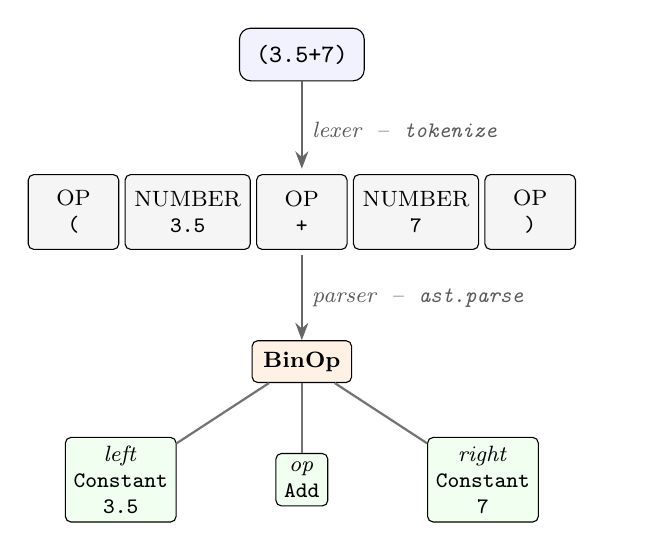
\begin{tikzpicture}[
  font=\footnotesize,
  >={Stealth[length=2.2mm]},
  src/.style={draw, rounded corners, fill=blue!5, inner sep=6pt, font=\ttfamily\small},
  tok/.style={draw, rounded corners=2pt, fill=black!4, align=center,
              minimum width=1.15cm, minimum height=0.95cm, font=\footnotesize},
  ast/.style={draw, rounded corners=2pt, fill=green!6, align=center, inner sep=3pt},
  root/.style={draw, rounded corners=2pt, fill=orange!10, align=center,
               inner sep=4pt, font=\bfseries\footnotesize},
  spine/.style={->, thick, black!60},
  tree/.style={black!55, thick},
  stagelbl/.style={font=\itshape\footnotesize, text=black!65},
]
% Stage 1: source
\node[src] (src) at (0,0) {(3.5+7)};
% Stage 2: tokens
\def\ty{-2.0}
\node[tok] (t1) at (-2.9,\ty) {OP\\\texttt{(}};
\node[tok] (t2) at (-1.45,\ty){NUMBER\\\texttt{3.5}};
\node[tok] (t3) at (0,\ty)    {OP\\\texttt{+}};
\node[tok] (t4) at (1.45,\ty) {NUMBER\\\texttt{7}};
\node[tok] (t5) at (2.9,\ty)  {OP\\\texttt{)}};
\node[font=\scriptsize, text=black!45, right=2mm of t5, align=left]
      {\quad};
% Stage 3: AST tree
\node[root] (binop) at (0,-3.9) {BinOp};
\node[ast] (left)  at (-2.3,-5.4) {\textit{left}\\\texttt{Constant}\\\texttt{3.5}};
\node[ast] (op)    at (0,-5.4)    {\textit{op}\\\texttt{Add}};
\node[ast] (right) at (2.3,-5.4)  {\textit{right}\\\texttt{Constant}\\\texttt{7}};
% pipeline arrows
\draw[spine] (src.south) -- (0,-1.45)
      node[stagelbl, right, pos=0.55] {lexer \;\textendash\; \texttt{tokenize}};
\draw[spine] (0,-2.55) -- (binop.north)
      node[stagelbl, right, pos=0.5] {parser \;\textendash\; \texttt{ast.parse}};
% tree edges
\draw[tree] (binop) -- (left);
\draw[tree] (binop) -- (op);
\draw[tree] (binop) -- (right);
\end{tikzpicture}%
} \caption{Lexing and parsing of the expression \texttt{(3.5+7)} in Python }
\label{fig:lex-parse}
\end{figure}

Lexical analysis simply means breaking down text into the smallest semantic units, ``tokens'', and analyzing them. The AST is a representation of the code as a tree, which allows for more depth (see Fig. \ref{fig:lex-parse}). The AST is what a compiler, transpiler, interpreter and most linters and formatters will consume (see Fig. \ref{fig:frontend-pipeline}).

% Preamble: \usepackage{tikz} +
\begin{figure}[t]
\centering
\resizebox{\columnwidth}{!}{%
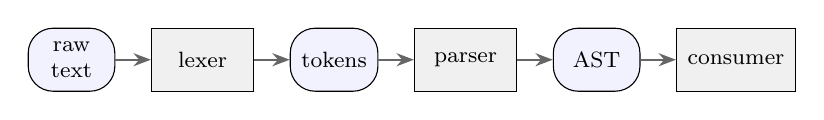
\begin{tikzpicture}[
  font=\footnotesize, >={Stealth[length=2.2mm]},
  data/.style={draw, rounded corners=9pt, fill=blue!5, align=center,
               inner sep=4pt, minimum height=8mm, minimum width=11mm},
  proc/.style={draw, fill=black!6, align=center,
               inner sep=4pt, minimum height=8mm, minimum width=13mm},
  ar/.style={->, thick, black!60}, node distance=4.5mm,
]
\node[data] (raw)               {raw\\text};
\node[proc, right=of raw] (lex) {lexer};
\node[data, right=of lex] (tok) {tokens};
\node[proc, right=of tok] (par) {parser};
\node[data, right=of par] (ast) {AST};
\node[proc, right=of ast] (con) {consumer};
\draw[ar] (raw) -- (lex); \draw[ar] (lex) -- (tok); \draw[ar] (tok) -- (par);
\draw[ar] (par) -- (ast); \draw[ar] (ast) -- (con);
\end{tikzpicture}}
\caption{Front-end pipeline of a static analyzer. \cite{aho2006compilers} Rounded nodes are data, rectangular nodes are processing stages.}
\label{fig:frontend-pipeline}
\end{figure}

\textbf{Examples}

\begin{enumerate}
    \item Syntax errors
    \item Name errors or misspellings
    \item Missing definitions and declarations
    \item Rule matching, e.g. leaked secrets
\end{enumerate}


\subsection{Type checking}

The idea behind types is that any data on a digital computer is simply some bitstring. The interpretation of this bitstring is what makes the data a value.

The data only makes sense if we define operations on it, but these operations depend on the type. For example, in Python the + operator for integers does integer addition, but for strings it does string concatenation. However, if you try to ``add'' an integer with a string, you get a type error. In Python type checking is done at runtime and is therefore called ``dynamic type checking''. However, for static analysis, we can check the types ahead of run-time, ``static type checking''. \cite{pierce2002tapl, python_datamodel}

In his paper ``A Theory of Type Polymorphism in Programming'' Robin Milner argues that well-typed programs cannot ``go wrong'' and that therefore programmers should use a formal type discipline. \cite{milner1978polymorphism}

\subsection{Flow Control}

A further class of semantic methods reasons about how information moves through a program. \emph{Information-flow analysis} tracks how the values of variables depend on one another, with the goal of certifying that secret data never reaches a public output. \cite{denning1977infoflow, sabelfeld2003infoflow} A flow from a variable $x$ to a variable $y$, written $x \rightarrow y$, means that observing $y$ may reveal something about $x$. Two kinds of such flows are distinguished. \cite{roth2025infoflow}

\subsubsection{\textbf{Explicit flows}} The most direct case is an assignment that copies a value. In the program $y := x$ all information from $x$ flows to $y$. The flow need not be total: in $y := \lfloor x/8 \rfloor$ not all, but some information may flow from $x$ to $y$, since $y$ no longer determines $x$ exactly. Both are \emph{explicit} flows, denoted $x \rightarrow y$, because the dependency is carried directly by the data passed in the assignment.

\subsubsection{\textbf{Implicit flows}} Information can also leak through the control flow itself, without any direct assignment from the source. Consider:

\begin{algorithmic}
\STATE $y := 0$
\IF{$x \geq 8$}
    \STATE $y := 1$
\ENDIF
\end{algorithmic}

Here $x$ is never assigned to $y$, yet some information still flows from $x$ to $y$: after the final line, observing $y$ tells us whether $x \geq 8$. This is an \emph{implicit} flow, again denoted $x \rightarrow y$. In general, any conditional control-flow change encodes information about the values that guided it, so a sound analysis must account for implicit as well as explicit flows. \cite{denning1977infoflow, sabelfeld2003infoflow}

\subsubsection{\textbf{Practical enforcement tools}} build on this distinction; the Jif/JFlow extension of Java, for example, lets programmers annotate data with security labels that the compiler then checks against both flow kinds. \cite{myers1999jflow}

\subsubsection{\textbf{Related flow-analysis techniques}} include control-flow analysis, which examines the possible paths of execution, and taint analysis, which follows untrusted (``tainted'') inputs to ensure they cannot reach sensitive operations unsanitized.

\subsection{Case study: Rust}

Rust is a low-level programming language started in 2006 by Graydon Hoare as a side project, then officially sponsored by Mozilla in 2009 and it finally reached maturity (v1.0) in 2015. Rust was specifically created to solve the flaws of C/C++. \cite{thompson2023rust, hoare2025rustdecade} This section tries to summarize how this is done in Rust.

``Who doesn't want memory safety, \emph{and} fast performance, \emph{and} a friendly compiler, \emph{and} great tooling, among a host of other wonderful features?'' \cite{klabnik2023trpl}

The Rust language has a very strict compiler which includes not just type checking but also a borrow checker and more. \cite{klabnik2023trpl} These checks lead to the conclusion that regular Rust code compiled through this strict compiler is also ``safe'': ``If it compiles, it works'' is common community lore. This recalls Milner's idea that well-typed programs cannot go wrong. \cite{milner1978polymorphism}

``Rust's type system and runtime guarantee the absence of data races, buffer overflows, stack overflows, and accesses to uninitialized or deallocated memory.'' \cite{matsakis2014rust}

The safety and soundness of a core subset of Rust was machine-checked in 2018 in the paper ``RustBelt: Securing the Foundations of the Rust Programming Language'', a formal soundness proof that also covers the encapsulation of well-typed \texttt{unsafe} code. \cite{jung2018rustbelt} These guarantees apply to \emph{safe} Rust; the \texttt{unsafe} escape hatch must be checked by hand, which is exactly what such proofs formalize.


% Not needed
% To make Rust more flexible, for example in very low-level settings without a standard library, "unsafe" Rust can be used. This allows for a small highly verified "unsafe" part and a general "safe" part. For example, linked lists without an allocator can only be implemented using "unsafe" code. "unsafe" code is not necessarily actually unsafe. The label rather points out that the code must be checked by hand, and, in contrast to "safe" code, the compiler cannot be relied on.

% On the other hand the compiler cannot always know all of our assumptions. For example, we don't have to care about race conditions in single-processor kernel code when interrupts are turned off. In these sitautions it also makes sense to use "unsafe" code.

\subsubsection{Case studies}
Large-scale industry data supports this: Microsoft reports that roughly 70\% of its annually assigned CVEs are memory-safety issues, \cite{miller2019bluehat, msrc2019saferlang}, while Android saw memory-safety vulnerabilities fall from 76\% to 24\% after shifting new development to memory-safe languages. \cite{vanderstoep2024android}


\section{Formal Methods}


``Classical static analysis finds symptoms; formal methods prove properties.'' Provable security is a desirable goal: it would, for example, remove the need to ship security patches at all. It also has real limitations, covered below.


\subsection{Formal Models and Formal Verification}
When applying formal methods, a formal model is created first; the kind of model depends on the use case. The desired properties are then checked against that model, for example by model checking, deductive verification (such as Hoare logic), or interactive theorem proving. This checking step is what is called formal verification.

\subsection{Hoare Logic}

Hoare logic is a program logic in which a fragment of code $C$ is annotated with a \emph{precondition} $P$ and a \emph{postcondition} $Q$, written as the Hoare triple
\[
  \{P\}\; C \;\{Q\}.
\]
Its meaning is that if $P$ holds before $C$ executes, then $Q$ is guaranteed to hold afterwards. For example,
\[
  \{x < 5\}\;\; \texttt{x += 1} \;\;\{x < 6\}.
\]

\subsubsection{\textbf{Loops}}
Loops are reasoned about through a \emph{loop invariant}: a property that holds before and after every iteration. For a \texttt{while} loop, the postcondition is the invariant conjoined with the negated loop condition, which necessarily fails once the loop terminates. A \texttt{for} loop can be \emph{unrolled} when its iteration count is statically known, or treated as an iteration over a data structure. For example Gaussian sum over \texttt{y} or mapping \texttt{*2} over a \texttt{list}:
\[
  \begin{array}{l}
    \{x = 0 \,\land\, y > 0\} \\[2pt]
    \quad \texttt{for i in range(y+1): x += i} \\[2pt]
    \{x = y(y+1)/2 \,\land\, y > 0\} \\[9pt]
    \{\,\forall i.\; x[i] \ge 0\,\} \\[2pt]
    \quad \texttt{for i in range(len(x)): x[i] *= 2} \\[2pt]
    \{\,\forall i.\; x[i] \ge 0\,\}
  \end{array}
\]

A \texttt{while} example computing the Gaussian sum makes the role of the invariant explicit:
\[
  \begin{array}{l}
    \{y \ge 0\} \\[2pt]
    \quad \texttt{x = 0; i = 0} \\[4pt]
    \textbf{inv}\;\; \{x = i(i+1)/2 \,\land\, i \le y\} \\[2pt]
    \quad \texttt{while i < y: i += 1; x += i} \\[4pt]
    \{x = y(y+1)/2\}
  \end{array}
\]
The invariant holds on entry (where $x = i = 0$) and is preserved by every iteration; on exit the loop condition fails, so $i = y$, and the invariant conjoined with this negated condition collapses to the postcondition $x = y(y+1)/2$.

\subsubsection{\textbf{Usage}} Hoare logic can be used to prove the correctness of algorithms which M. Foley and C.A.R. Hoare demonstrated quite nicely in ``Proof of a Recursive Program: Quicksort'' (1971). \cite{foley1971quicksort}

\subsection{Overview of Methods and Tools}

\begin{enumerate}
    \raggedright
    \item Model-based formal specification languages~\cite{iotformalreview2024} like Z~\cite{spivey1992z}, the Vienna Development Method (VDM)~\cite{jones1990vdm}, and B~\cite{abrial1996bbook}
    \item Interactive proof assistants~\cite{dafny2026workshop} like Rocq (formerly Coq),\cite{rocq2025} Isabelle/HOL~\cite{nipkow2002isabelle} or Lean~\cite{demoura2015lean}
    \item Verification-aware programming languages~\cite{dafny2026workshop} like Dafny~\cite{leino2010dafny}, SPARK~\cite{mccormick2015spark}, F*~\cite{swamy2016fstar}, Why3~\cite{filliatre2013why3}, Viper~\cite{mueller2016viper}, Whiley~\cite{pearce2013whiley} or hax~\cite{bhargavan2025hax}
    \item Crypto verifiers like ProVerif~\cite{blanchet2001proverif} and EasyCrypt~\cite{barthe2011easycrypt}
\end{enumerate}

\subsection{Examples}

\subsubsection{\textbf{Z}}

The Z notation (pronounced ``zed'') is a formal specification language for describing and modelling computing systems~\cite{spivey1992z, z_wiki}. It uses mathematics, mainly sets and logic, to write a precise, unambiguous description of what a system should do, before any code is written. Its main building block is the \emph{schema}: a named box that groups some variables together with rules about how they may behave, and schemas can be combined to build up larger specifications. Z is not executable; it describes a system rather than implementing it. It has been applied to real industrial systems, most famously the formal specification of IBM's CICS transaction-processing software, work that earned Oxford University and IBM a Queen's Award for Technological Achievement in 1992.

\subsubsection{\textbf{Dafny}}

In the original paper on Dafny, Leino gave the challenges of directly using interactive proof assistants and satisfiability-modulo-theories (SMT) solvers as main reason for the creation of Dafny. The idea is that the programmer doesn't have to interact with any proof assistant or solver directly, only needs to make certain annotations. The original paper shows the simple usage: You define a \texttt{method} and pre- and postconditions (see Fig.~\ref{fig:dafny-isqrt}), just like in Hoare logic. \cite{leino2010dafny}.

Dafny also compiles down to C\#, Java, JavaScript, Go, and Python. A more complete algorithm for creating the Dutch flag can be found in Fig. \ref{fig:dafny-full}. \cite{dafny_org}.


\begin{figure}[t]
\centering
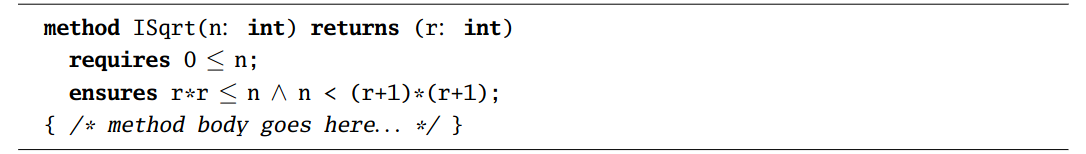
\includegraphics[width=\columnwidth]{dafny.png}
\caption{A Dafny method specification: \texttt{ISqrt} returns the integer square
root \texttt{r} of a non-negative input \texttt{n}~\cite{leino2010dafny}.}
\label{fig:dafny-isqrt}
\end{figure}

\begin{figure}[t]
\centering
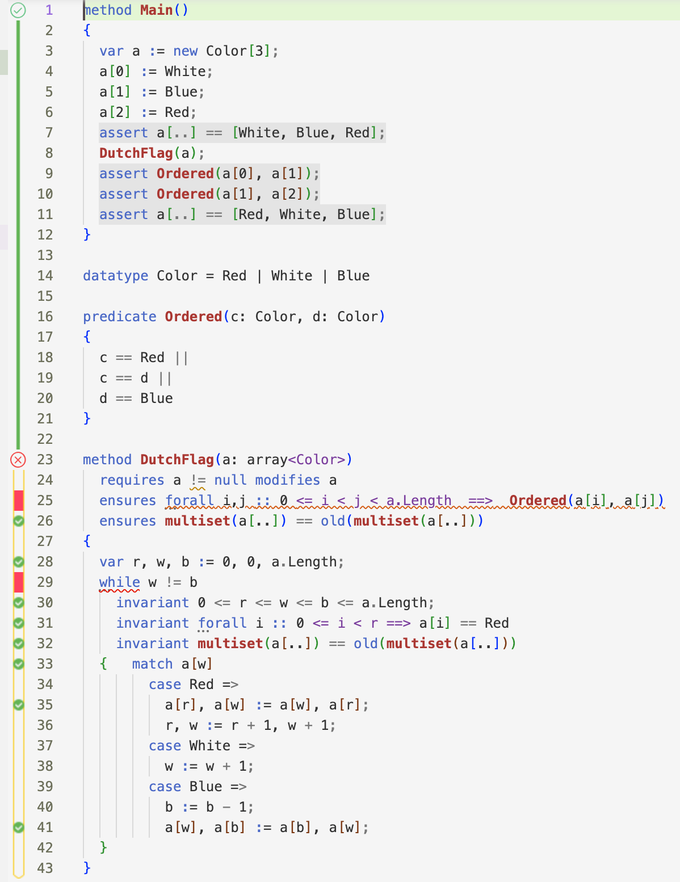
\includegraphics[width=\columnwidth]{dafny-full.png}
\caption{A fully verified Dafny program (the Dutch national flag); the IDE gutter
shows the per-line verification status~\cite{dafny_org}.}
\label{fig:dafny-full}
\end{figure}

\subsubsection{\textbf{hax}}

Hax is a tool for proving code written in Rust. It translates a large (though not complete) subset of Rust into formal languages such as F* or Rocq, where security properties and functional correctness can then be discharged with the appropriate prover~\cite{bhargavan2025hax, hax_cryspen}.

\begin{figure}[t]
\centering
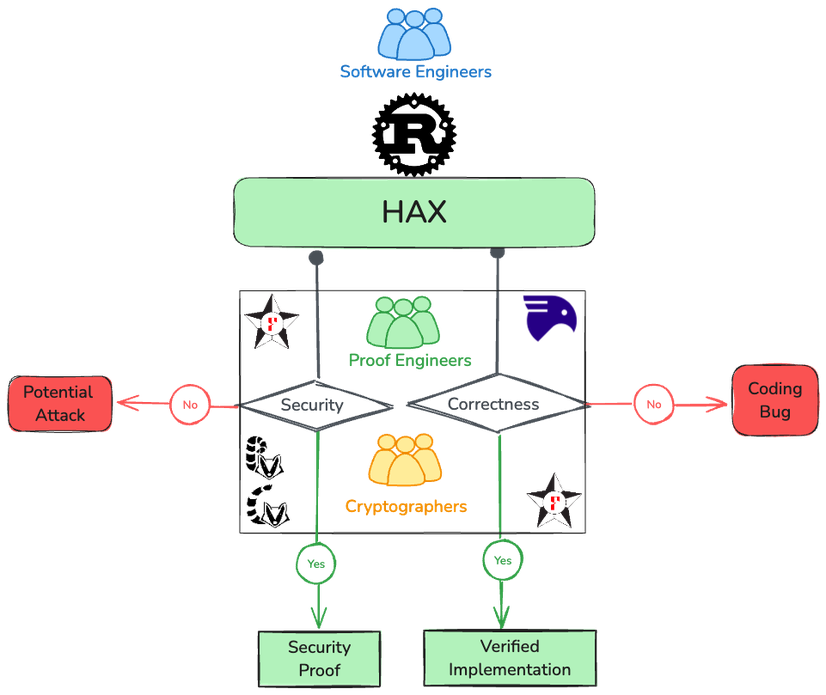
\includegraphics[width=\columnwidth]{hax.png}
\caption{The hax workflow: Rust code is routed through hax to separate
security and correctness proofs, each verified via prover backends~\cite{hax_cryspen}.}
\label{fig:hax}
\end{figure}

Hax is a verification toolchain aimed at security-critical software such as cryptographic libraries, protocol implementations, and parsing or sanitization code. Its guiding observation is that different verification tools excel at different goals, so rather than committing to a single prover it extracts the supported subset of a Rust program and translates it into the input language of whichever backend fits the property at hand: domain-specific security analyzers like ProVerif for protocol- and cryptography-level security arguments, and general proof assistants like F* and Rocq for functional correctness. Because soundness then rests on these translations, the authors systematically test both the generated models and their models of the Rust system libraries against the original code. \cite{bhargavan2025hax}

A flagship application of this toolchain is Bertie (``Bert13''), a portable post-quantum TLS~1.3 implementation in Rust that hax verifies using F*, ProVerif, and SSProve for runtime safety, parsing correctness, and protocol security. \cite{bhargavan2025bertie}

\subsubsection{\textbf{ProVerif}}

ProVerif is a tool for the automatic, symbolic verification of cryptographic protocols~\cite{blanchet2001proverif, proverif_web}. It works in the Dolev-Yao model, in which cryptography is assumed to be perfect and treated as a black box, while the attacker is given full control of the network: messages can be intercepted, modified, replayed, or injected, but the encryption itself cannot be broken. Given a description of a protocol, ProVerif checks security properties such as secrecy (whether an attacker can learn a secret value) and authentication. It has been used to verify and improve real-world protocols, including Signal, TLS, avionic protocols, and internet voting. Unlike Dafny or hax, which reason about the correctness of code, ProVerif reasons about the security of a protocol's design, which is why hax can target it as one of its backends~\cite{bhargavan2025hax}.

% To have a smooth transition to the next chapter, i.e. motivate using LLMs
\subsection{Limitations}

Despite these successes, a recent comprehensive review of formal methods for IoT identifies several recurring gaps that still limit their adoption~\cite{iotformalreview2024}:

\begin{itemize}
  \item \textbf{Scalability.} As IoT networks grow, so does the state space a verifier must explore; techniques such as model checking quickly run into state-space explosion and become computationally infeasible for large-scale deployments.
  \item \textbf{Real-time performance.} Formal methods do not yet fully capture the timing behavior of IoT systems, where processing delays and network latency threaten strict deadlines, a serious obstacle in time-sensitive domains such as healthcare and industrial automation.
  \item \textbf{Cooperation between methods.} Model checking, theorem proving, and formal specification have complementary strengths, but there is little work on integrating them; the absence of frameworks that combine these techniques prevents holistic verification of both functional and non-functional requirements.
  \item \textbf{Adaptability.} IoT systems evolve constantly as devices are added, updated, or removed, whereas most formal models are static and cannot track such changes without full re-verification.
  \item \textbf{Security and privacy.} Much of the literature concentrates on functional correctness, leaving security- and privacy-specific properties comparatively under-addressed despite the sensitivity of IoT data.
  \item \textbf{Usability.} The mathematical intricacy of formal methods keeps them out of reach for most practitioners; more accessible, developer-friendly tooling is needed before they see widespread industrial use.
\end{itemize}

\section{Artificial Intelligence\\ for Formal Verification}\label{sec:ai}

The usability and scalability gaps just described have made formal verification a natural target for machine learning. Deep-learning methods, and more recently LLMs, are now applied across the proving workflow, from autoformalization and premise selection to generating individual proof steps and searching for whole proofs~\cite{li2024dltp}. The appeal follows directly from the barrier identified above: if a model can supply the tedious invariants, annotations, and proof scripts that formal tools demand, verification becomes accessible to developers who are not themselves proof experts. A prominent demonstration is AlphaProof, an AlphaZero-style agent that learns to write formal Lean proofs through reinforcement learning and, together with AlphaGeometry~2, reached silver-medal-level performance at the 2024 International Mathematical Olympiad~\cite{hubert2025alphaproof}.

The pairing of AI with formal methods is complementary in both directions. LLMs are powerful but non-deterministic: they produce plausible proofs or code with no guarantee of correctness. A formal verifier supplies what they lack, a deterministic oracle that either accepts a proof or rejects it with a concrete error. It grounds the model's output in a checkable truth and closes a tight feedback loop, since the prover's error can be fed straight back as the next prompt until the proof checks. Because soundness rests on the verifier rather than the model, an unreliable generator can still yield a trustworthy result, but only relative to the specification it is checked against. This caveat matters: a proof of a wrong or vacuous specification is worthless, and models are known to ``game'' the checker by weakening postconditions or inserting unproven assumptions, a failure mode that recent evaluations document explicitly~\cite{bayazit2025casestudy}. Writing a correct, complete specification is itself hard, and where the model is asked to supply the specification as well as the proof~\cite{misu2024dafny} the verifier only checks the code against the model's own claim, so the guarantee becomes circular. The residual difficulty therefore moves to the specification: a developer who is not a verification expert may be unable to distinguish a faithful specification from a weakened one, so for that audience these tools shift the effort from writing proofs to reviewing specifications rather than removing it. In the other direction, formal modelling is notoriously tedious; hand-writing specifications, invariants, and proof scripts is much of why these techniques, despite their guarantees, are so seldom used in practice. That is the kind of laborious, pattern-heavy work LLMs handle well, so a model can take on the bulk of it and leave the engineer to supervise, easing the usability gap identified earlier.

\subsection{Case studies}

Most current work attaches an LLM to an existing verifier and asks it to produce the artifacts that verifier needs. For Rust checked with the Verus tool, Yao et al.\ combined GPT-4 with static analysis to synthesize the loop invariants and assertions Verus requires, easing the proof burden on small programs~\cite{yao2023rustproof}. AutoVerus scales this idea up with a network of orchestrated LLM agents that imitate an expert's generate, refine, and debug loop, solving more than 90\% of a 150-task benchmark~\cite{yang2024autoverus}.

Dafny has received comparable attention. Misu et al.\ ran the first empirical study of prompting LLMs to synthesize Dafny methods \emph{together with} their formal specifications~\cite{misu2024dafny}, while Laurel uses domain-specific prompting to generate the helper assertions Dafny's SMT backend needs, recovering roughly 56\% of the assertions in a real-world dataset~\cite{mugnier2024laurel}.

In interactive proof assistants the unit of automation is larger. Baldur fine-tunes an LLM to generate entire Isabelle/HOL proofs in a single shot, and then to repair them from the prover's own error output, outperforming search-based methods~\cite{first2023baldur}. PALM takes a generate-then-repair approach for Coq, pairing the model with symbolic tactics to close proofs it cannot produce directly~\cite{lu2024proofauto}.

Closest to the security-critical setting of this report, a recent experience report revisits the hax toolchain seen earlier but replaces its classical backends with AI provers. It translates production Rust cryptographic code (zkEVM primitives in Plonky3 and RISC~Zero) into Lean~4, recording which proof obligations the AI could discharge and where human effort was still required~\cite{klaus2026rustlean}. Where Bertie verifies a complete TLS stack with classical provers, this pipeline probes how far AI provers can carry the same toolchain on real code.

These results are encouraging, but they are largely measured on benchmarks. DafnyBench, a suite of roughly 750 programs, reports a best success rate near 68\% for LLM-generated verification hints~\cite{loughridge2024dafnybench}. On the genuinely large, Coq-verified FSCQ file system, however, the same class of models reproduces only about 38\% of the proofs, with scale and lemma retrieval becoming the bottleneck~\cite{qin2025fscq}; a broader case study across proof assistants reaches the same conclusion, cataloguing the many distinct failure modes current models exhibit~\cite{bayazit2025casestudy}. This mirrors the industrial static-analysis experience seen earlier: a benchmark score and the behavior on real, security-critical code can differ sharply, and for IoT it is the real-code behavior that matters.

\section{Discussion}

Formal verification tools and, more generally, static analysis tools are mostly ``solved'', in the sense that the ideas still in practice today are from the late 1960s to the 1980s. \cite{hoare1969axiomatic, cousot1977ai, denning1977infoflow} The things that change are the applications, programming languages and the ease-of-use.

For formal verification to become more widely adopted, not only must ease-of-use improve, but legal requirements, standards, and consequences must increase as well. Recent measures push in this direction: the EU Cyber Resilience Act, which mandates security-by-design and vulnerability handling for connected products and backs them with substantial fines, and consumer-IoT baselines like ETSI EN 303 645. \cite{eu2024cra, etsi2024en303645} Until such requirements and their consequences are stronger, the incentives are simply not enough.

However, LLMs and new more advanced auto-solvers like hax~\cite{bhargavan2025hax} or Dafny~\cite{leino2010dafny} provide the possibilities to prove more-and-more and larger-and-larger codebases. One limitation that is still open however is the \textbf{cooperation between methods}~\cite{iotformalreview2024} and the \textbf{hardware interoperability}.

For cooperation, tools like hax and Dafny that think this abstraction from the beginning, are very valuable: hax compiles Rust to several verification systems~\cite{hax_cryspen} and Dafny compiles to several different programming languages~\cite{dafny_org}. They are therefore already highly adaptable.

To adapt better to hardware specifics, one direction is to specify the hardware itself in a formal language rather than emulating it with tools like QEMU, a kind of \emph{theoretical emulator}, so that the same model serves both execution and proof. This is not hypothetical: architecture-definition languages such as Sail already generate both executable emulators and proof-assistant models of an instruction set (e.g.\ ARM and RISC-V) from a single formal specification~\cite{armstrong2019sail}; the open problem is extending this style of hardware/software co-verification to the heterogeneous, constrained processors typical of IoT.

\section{Conclusion}

This report followed a single question across three families of technique: how can we gain confidence that software is correct and secure \emph{before} it runs? The question is highly relevant to IoT, whose tens of billions of devices are often too numerous to supervise, too constrained to defend at runtime, and too rarely updated to fix after the fact. 

Static analysis sits at one end of the spectrum. It is relatively cheap and fast, and it can flag whole classes of defect, from syntax and type errors to information-flow leaks, without ever executing a line. Its reach has grown from lexical checks over token streams to semantic reasoning about types and data flow, and languages such as Rust now push much of it into the compiler itself, making memory-safety errors unrepresentable by construction. Yet the main lesson from deploying these tools at industrial scale is not about analytical power at all: Coverity, Google, and Facebook each found that adoption hinges on low false-positive rates and tight integration into the developer's workflow.

Formal methods sit at the other end; they \emph{prove} the absence of whole classes of fault instead of just flagging symptoms. Hoare logic shows how a precondition, a program, and a postcondition can be tied into a checkable guarantee, and modern verification-aware languages turn that idea into practical tooling: Dafny discharges proof obligations through an SMT backend, while hax carries security-critical Rust into provers such as F* and Rocq, the foundation on which the Bertie post-quantum TLS stack was fully verified with no language models in the loop. The catch, once again, is adoption. A recent review of formal methods for IoT catalogues six recurring gaps: scalability, real-time behavior, cooperation between methods, adaptability, a thin focus on security and privacy, and, above all, usability. It is the sheer tedium of hand-writing specifications and proofs that keeps these guarantees out of everyday practice.

Language models are now being applied to exactly this gap. In only a few years LLMs have gone from solving almost none of the SWE-bench issues to nearly all of them, and a related, more demanding, generative ability is now being turned on verification itself: tools such as AutoVerus, Laurel, Baldur, and PALM let a model supply the invariants, assertions, and proof scripts that formal engines demand. The pairing helps both sides: the model gains a deterministic oracle to check against, and in return it absorbs the tedious annotation work that made formal methods unpalatable. Soundness still rests on the verifier rather than the model, so even an unreliable generator can yield a trustworthy result, as long as the specification it is checked against is correct. The honest caveat is that today's strong numbers are mostly benchmark numbers: on genuinely large, security-critical code such as the FSCQ file system the success rate falls sharply, the benchmark-versus-reality gap that the static-analysis case studies warned about.

A promising path for IoT is to combine techniques rather than rely on any one: the productivity of AI together with the soundness of a formal engine, which would lower the usability barrier that has long kept verification away from constrained, unpatchable devices. Two problems remain: First, the evidence is not sufficient: results are strong on small benchmarks but fall off sharply on large, real systems, and none of the AI-assisted verification surveyed here has yet been demonstrated on IoT firmware, so this is a direction rather than a settled result. Second, usability is necessary but not sufficient for adoption: as the introduction argued, IoT insecurity is driven as much by economic incentives and an unpatchable installed base as by the cost of proof, and development-time verification helps only the devices still to be built. With those caveats, the tools best placed to exploit this composition are those built for cooperation from the start, such as hax compiling Rust to several provers and Dafny compiling to several languages. The remaining frontier is the boundary with hardware, where formal models of an instruction set in the spirit of Sail could one day let software and hardware be verified against a single specification. Almost none of the underlying theory is new; the lexical, type-theoretic, flow-based, and Hoare-style ideas surveyed here date from the late 1960s to the 1980s. What is finally changing is their ease of use. On its own, cheaper proof will not move an industry whose incentives point elsewhere; but combined with the legal and economic pressure discussed above, lowering the cost of correctness is a necessary part of any durable solution for IoT devices that cannot be patched into safety.

\section{Use of AI}

\begin{enumerate}
  \item Used Perplexity for research (i.e. finding papers).
  \item Used ChatGPT and Claude to suggest a finer outline: https://claude.ai/share/a1e3b8b4-a6da-4b14-85c9-6de0babfcf5e
  \item Used Claude for help with LaTeX: installation, auto-compile setup, errors, figures and layout
  \item Used Claude to find citations for things I only know in my head -> had to be thoroughly verified because it likes to make stuff up
  \item Finally, I used Claude for a paper review and language rewrite (e.g. more formal tone)
\end{enumerate}

For search, AI search is simply the next level of Google search or similar. Other tasks are either tedious nuisances that have no scientific value (e.g. setting up LaTeX) or are tasks that other humans would do (review and checking citations). In general I tried to make sure the AI is not driving my work (the extreme of which would look like this: write me an article on topic X), but I am driving the AI and simply using it as a more advanced tool and partner.  


\bibliographystyle{IEEEtran}
\bibliography{references}
\vspace{12pt}

\end{document}
